\chapter{Results}
\label{chap:3}
\ChapterPageStuff{3}

\section{Introduction}
In \Cref{sec:ch2_preamble}, the methodology was created for a web-based software system. As described in this section, a user can have multiple systems and subsystems linked to their account. The implementation is done for multiple software systems in this section. The system implementation will focus more on the development of the logging mechanism, and the critical analysis will prioritise software maintenance using a utilisation analysis.

\section{Implementation and verification}
In this sections the implementation of the development of solution will be discussed using a test system to verify it. The test system is created in a \texttt{ASP.NET COre Web SDK} software environment.

\subsection{User activity types}
For the test system the basic use will be:

\begin{itemize}
	\item monitor reasource usage dynamic dashboards,
	\item generate \texttt{PDF} reports of the displayed data.
\end{itemize}

Reporting and monitoring are important for this test system so the user activity types will need to focus on these activty types.

\begin{table}[!htb]
	\centering
	\caption[Test user activity types]{\textit{Test user activity types}}
	\label{tbl:ch3_testActivityTypes}
	\begin{tabularx}{\textwidth}{|X|l|X|}
		\hline \textbf{Activity} & \textbf{Functional requirement} & \textbf{Description} \\
		\hline \texttt{SystemAccess} & \ref{fr:uatType1} & \RaggedRight This actvity type detects when a user has navigated to a certain subsystem. \\ 
		\hline \texttt{General} & \ref{fr:uatType3} & \RaggedRight This general actvity type is for all other actviities that user initiates that send \textit{HTTP request} back to the server. \\
		\hline \texttt{ReportExport} & \ref{fr:uatType3} & \RaggedRight The other main functionality of the system is for reporting purposes. Seperating this type of actvity in its own category to capture all report generation actvities that the user initiated. \\ 
		\hline
	\end{tabularx}
\end{table}

\Cref{tbl:ch3_testActivityTypes} doesn't contain any session changes (\ref{fr:uatType3}) user types. These actviities is only trigger when the user log's into their system or terminate their session by pressing the log out button.

\clearpage

\subsection{Log attibutes}\label{sec:ch3_logAtrributes}
Using the functional requirements discussed in \Cref{sec:ch2_logAttributesRequirements} data columns is made for the user based event's log attributes. These log attributes for a structured database are defined in \Cref{tbl:ch3_Log_Attributes}. 

\begin{table}[!htb]
	\centering
	\caption[Logging attributes]
	{\textit{Logging attributes}}
	\label{tbl:ch3_Log_Attributes}
	\begin{tabularx}{\textwidth}{|l|l|X|}
		\hline \textbf{Column name} & \textbf{Requirement ID} & \textbf{Description}\\
		\hline \texttt{ID} & \ref{fr:lpa1} & User based actvity primary identifier. \\
		\hline \texttt{TimeStamp} & \ref{fr:lpa2} & Date timesstamp when the activity has occur. \\
		\hline \texttt{ActivityType} & \ref{fr:lpa3} & Activity type of the log event. \\
		\hline \texttt{UserId} & \ref{fr:lpa4} & Identification number of the user associated with the log event. \\
		\hline \texttt{SystemId} & \ref{fr:lpa5} & System where the activity has occur. \\
		\hline \texttt{SubsystemId} & \ref{fr:lpa5} & Subsystem where the activity has occur. \\
		\hline \texttt{MetaData} & \ref{fr:lpa6} & Metadata captured from the \textit{HTTP request}. \\
		\hline \texttt{ClientId} & \ref{fr:lpa7} & Additional identifiers for the log event. In this case different configuration of the same system for a specific client. \\
		\hline
	\end{tabularx}
\end{table}

The data columns in \Cref{tbl:ch3_Log_Attributes} is used in structured database which is \texttt{MySQL} database. This database have pre existing tables that expand on other data such as the \texttt{UserId}, \texttt{SystemId} and \texttt{SubSystemId}. For the \texttt{MetaData} the \texttt{JSON} is similar to \Cref{fig:ch3_MetadataJson}.

\begin{lstlisting}[style=json, caption={\textit{Metadata JSON}}, label={fig:ch3_MetadataJson}] 
	{
		"RequestOrigin": "/System/Subsystem1/GetData",
		"RequestElementID": "ButtonSaveCsv",
		"RequestParameters": {
			"aTagIDs": [
				"6284",
				"20320"
			],
			"aToDate": "2020-04-06",
			"aGroupID": 2,
			"aFromDate": "2020-03-30"
		}
	}
\end{lstlisting}

In \Cref{fig:ch3_MetadataJson} the main \texttt{JSON} parameters captures the following additional data for the user based event:

\begin{itemize}
	\item \texttt{RequestOrigin} is the full file path of the subsystem that is being used and function to fullfil the \textit{HTTP request}. Some of the subsystems consist of multiple individual files and this traces the origin of the \textit{HTTP request} function user based actviity accessed.
	\item \texttt{RequestElementID} is the last \textit{HTTP} element identifircation that the user interacted with that intiated the user based actvity.
	\item \texttt{RequestParameters} is the request parameters that are send with the \textit{HTTP request}. Any sensitive user data is either igonred by adding flags to certain subsystems or individual functions to not obtain the request's parameters.
\end{itemize}

\subsubsection{Obtaining the element of user-based event}\label{sec:ch2_ElementObtaining}
In \Cref{sec:ch2_webApplicationArchitecture} the user-based activity event will be use a \textit{HTTP request} to send to the server when the user interacted with an \textit{HTML element}. For the functional requirements activity type (F/R 1.5.3) and metadata (F/R 1.5.6) in \Cref{tbl:ch2_keyLoggingAttributes} the \textit{HTML element} needs to be obtained to get the element's tag and identification text. This can be difficult to obtain due to \textit{bubbling}\footnote{\textbf{Bubbling} is when an event happens on an element, it first runs the handlers on it, then on its parent, then up on other ancestors. \cite{EventBubbling}.} that may occur when searching for the element that the user specifically interacted with.\par In \Cref{fig:ch2_event_bubbling} is the event propagation example of a child element that has been clicked on which executes a DOM event. The event propagation consists of three phases~\cite{EventBubbling}:

\begin{itemize}
	\item \textit{Capturing phase:} The event propagates downwards to the targeted element that the user interacted with.
	\item \textit{Target phase:} The event reaches the targeted element to execute the DOM event.
	\item \textit{Bubbling phase:} The event bubbles up from the targeted element
\end{itemize}

\begin{figure}[!htb] % An h :here, t: top, b: bottom.
	\centering % cent the figure
	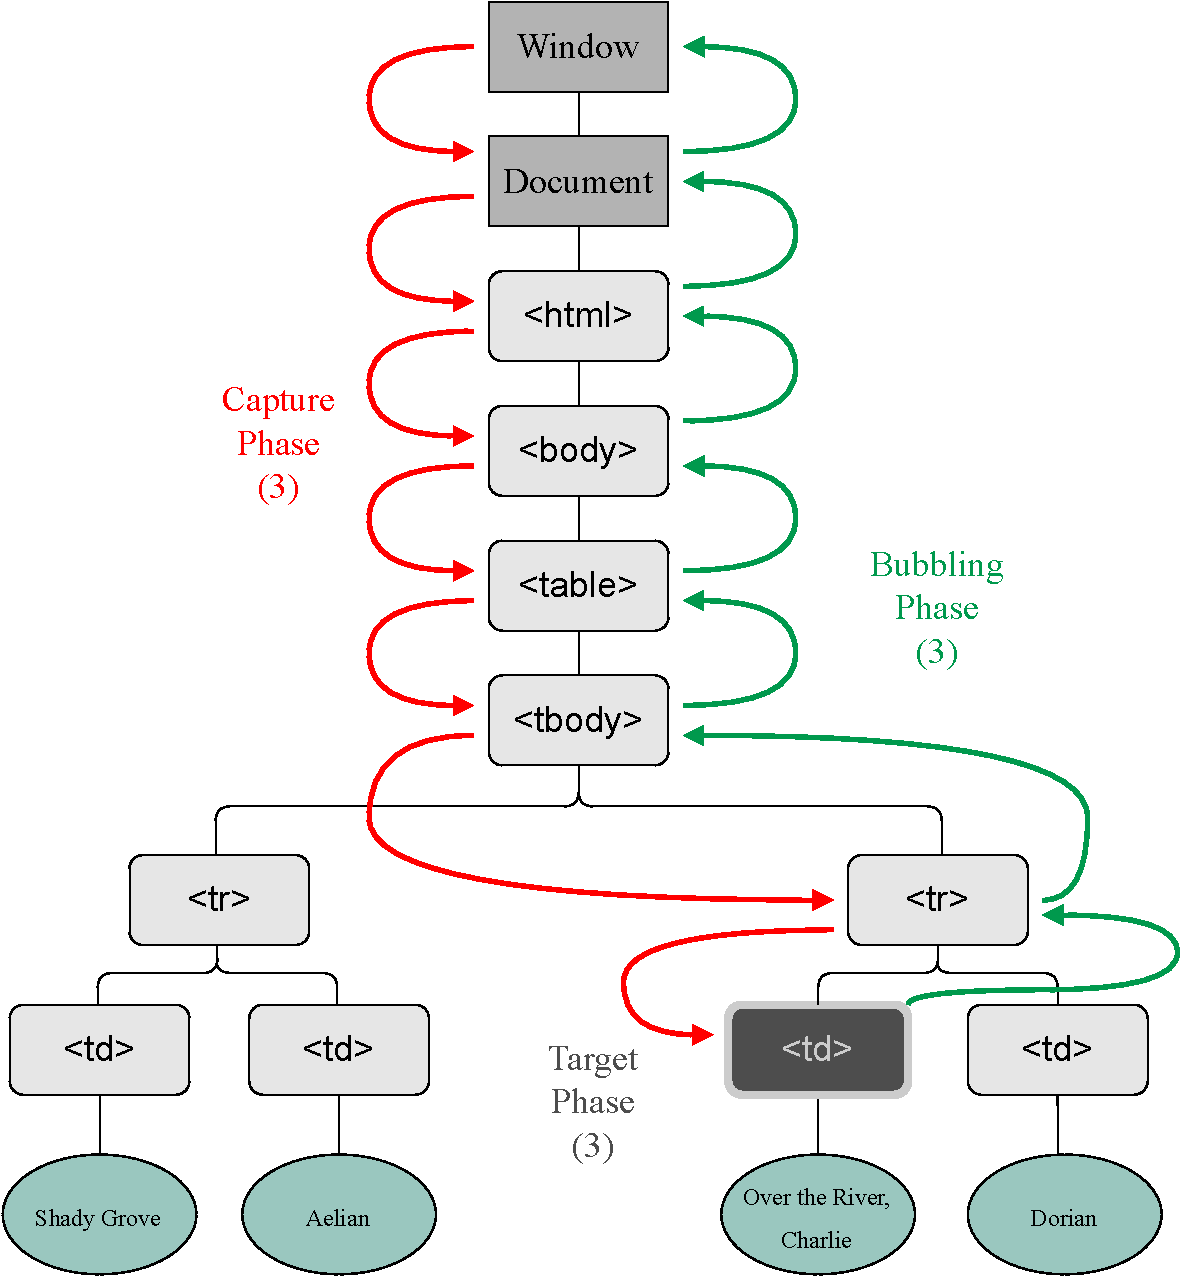
\includegraphics[width=0.6\textwidth]{Chapter2/event_bubbling/event_bubbling.pdf}
	\caption[JavaScript event propagation]
	{\textit{JavaScript event propagation~\cite{EventBubbling}}}\label{fig:ch2_event_bubbling}
\end{figure}

Capturing the targeted element may be difficult as some web pages may have more complex HTML, which can cause event propagation to fail to obtain the correct element information that the user interacted with. In such cases, it is more accurate to obtain the targeted element by identifying the last known element that the user hovered over on the user interface, as another DOM event may have started during the initial element's event.\par \Cref{fig:ch2_element_event_capturing} shows the flow diagram to capture the element that the user interacted with for the user-based activity log. This code segment will be initiated during the \texttt{beforeSend} operation of the \textit{AJAX request} to filter HTML elements by predefined allowed elements. Filtering the element tag names ensures that unwanted, more complex elements or basic elements that are not expected to be the initiator of the event, will be excluded.\par If the web location has already changed or no element exists, it is possible that the contents of the page have already changed during the event propagation. Therefore, the last known element that the user hovered over must be used, as it is most likely to be the element that the user interacted with. This approach ensures that there is always an element that has been detected and parsed with the request header in most UI changes.


\begin{figure}[!htb] % An h :here, t: top, b: bottom.
	\centering % cent the figure
	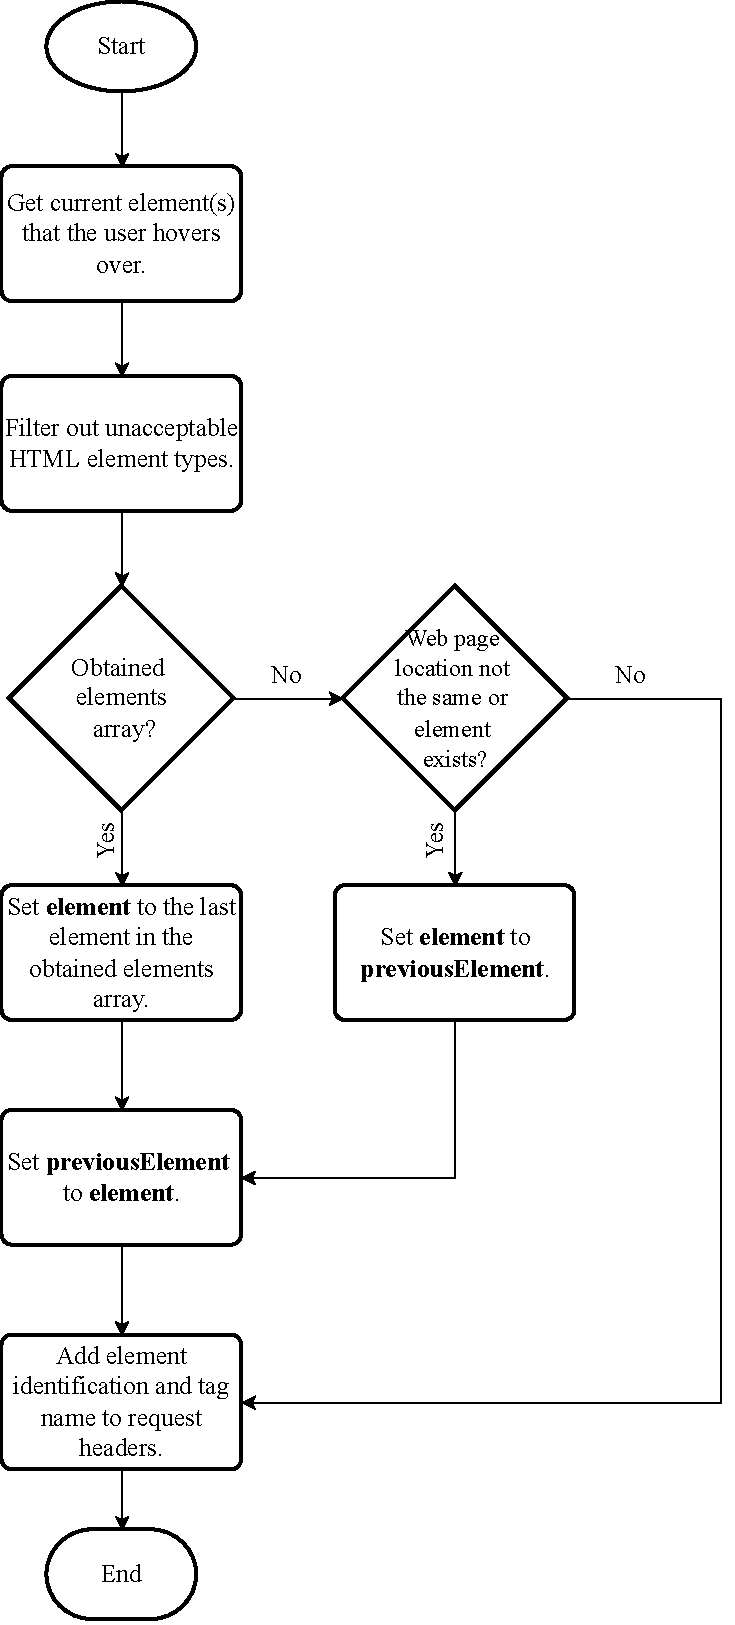
\includegraphics[width=0.6\textwidth]{Chapter2/element_capturing/element_capturing.pdf}
	\caption[HTML element capturing flow diagram]
	{\textit{HTML element capturing flow diagram}}\label{fig:ch2_element_event_capturing}
\end{figure}

\clearpage


    \begin{xltabular}{\textwidth}{|X|X|X|X|X|X|X|}
        \caption[Test data]
        {\textit{Test data}}
        \label{tbl:apx_testB_Normilised} \\
        
        \hline
        \textbf{$S_{X}$} & \textbf{$P_X$} & \textbf{$P_N$}  & \textbf{$A_X$} & \textbf{$A_N$} & \textbf{$M_{PF}$} & \textbf{$P_{R}$} \\
        \hline
        \endfirsthead

        \multicolumn{7}{c}
        {\tablename\ \thetable{} -- continued from previous page} \\
        \hline
        \textbf{$S_{X}$} & \textbf{$P_X$} & \textbf{$P_N$}  & \textbf{$A_X$} & \textbf{$A_N$} & \textbf{$M_{PF}$} & \textbf{$P_{R}$} \\ 
        \endhead

        \multicolumn{7}{|r|}{{Continued on next page}} \\ \hline
        \endfoot

        \hline
        \endlastfoot
    $S_1$ & 226 & 0.6504 & 11 & 0.8333 & 0.5420 & 1 \\ \hline
 $S_2$ & 269 & 1.0000 & 5 & 0.3333 & 0.3333 & 2 \\ \hline
 $S_3$ & 156 & 0.0813 & 8 & 0.5833 & 0.0474 & 3 \\ \hline
 $S_6$ & 154 & 0.0650 & 8 & 0.5833 & 0.0379 & 4 \\ \hline
 $S_4$ & 155 & 0.0732 & 1 & 0.0000 & 0.0000 & 5 \\ \hline
 $S_5$ & 146 & 0.0000 & 13 & 1.0000 & 0.0000 & 5 \\ \hline
    \end{xltabular}
    

\section{Verification}

\begin{landscape}
	\begin{figure}[!htb] % An h :here, t: top, b: bottom.
		\centering % cent the figure
		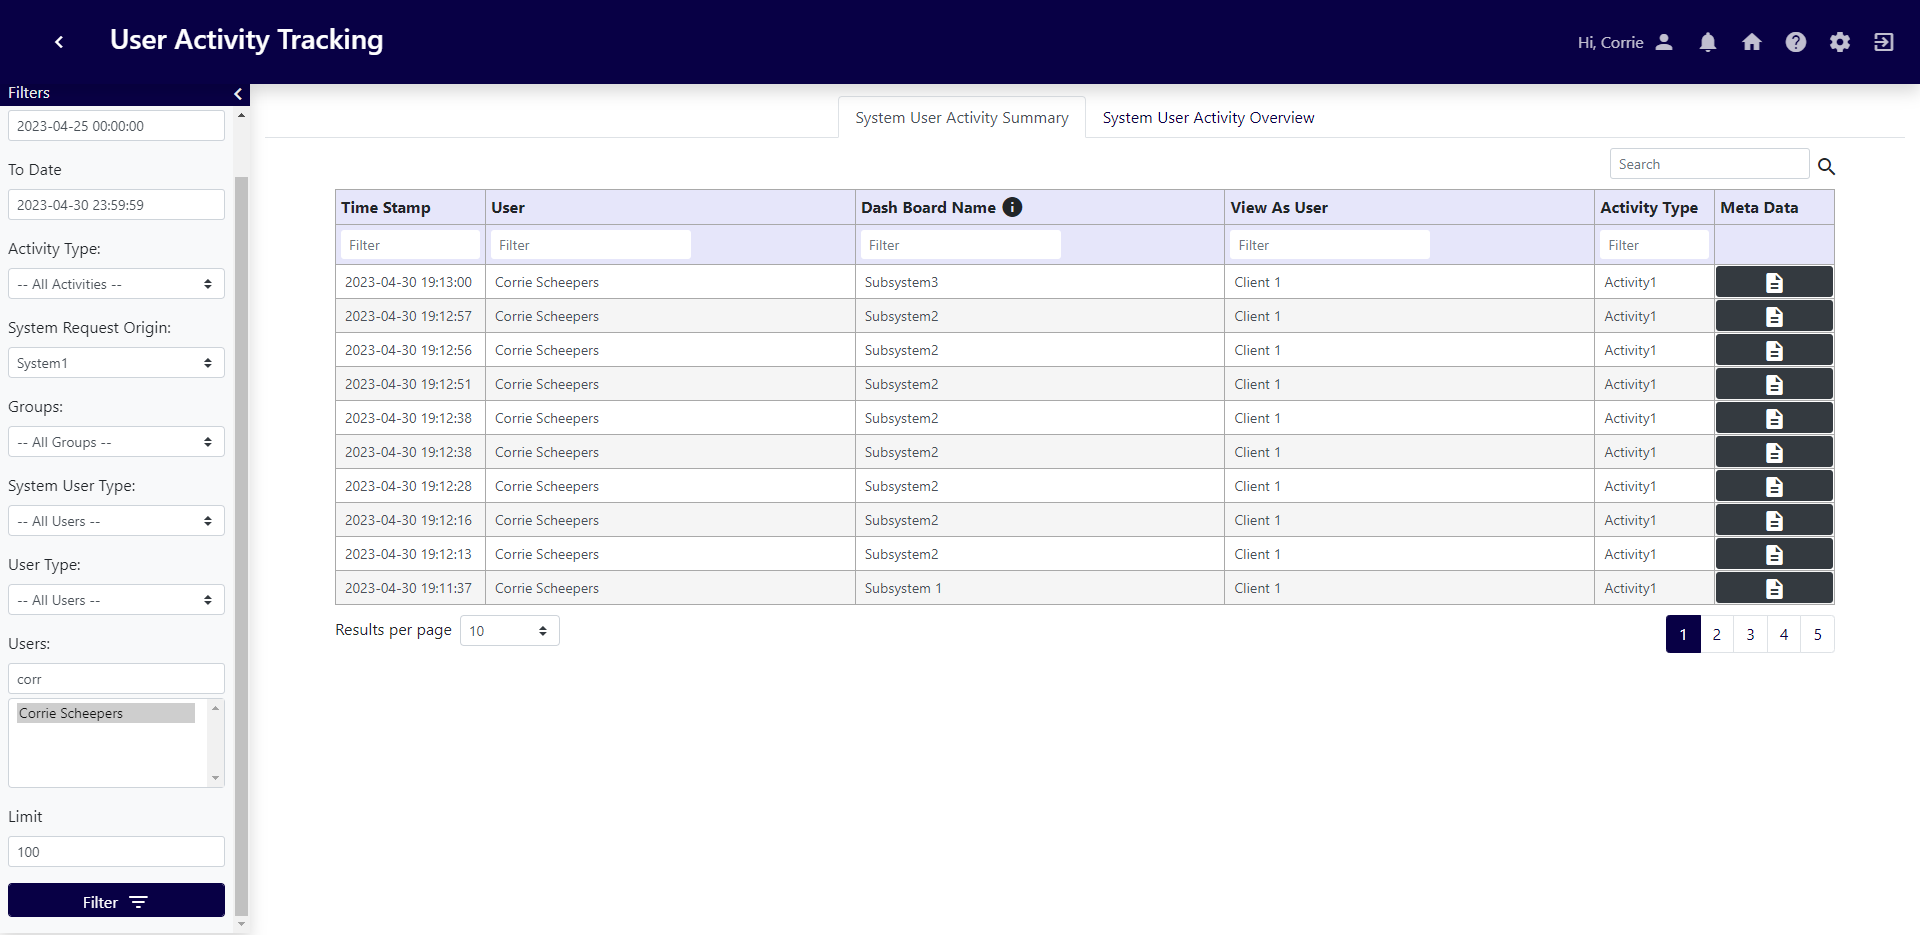
\includegraphics[width=0.99\linewidth]{img/ch3/analysis/UAT_menu.png}
		\caption[Interactive user actvity viewer]
		{\textit{Interactive user actvity viewer}}\label{fig:ch3_UAT_menu}
	\end{figure}
\end{landscape}

\section{Case studies}

\subsection{Case study identification}

\subsection{Case study results}

\subsubsection{System A results}

\begin{landscape}
	\begin{figure}[!htb]
		\centering % cent the figure
		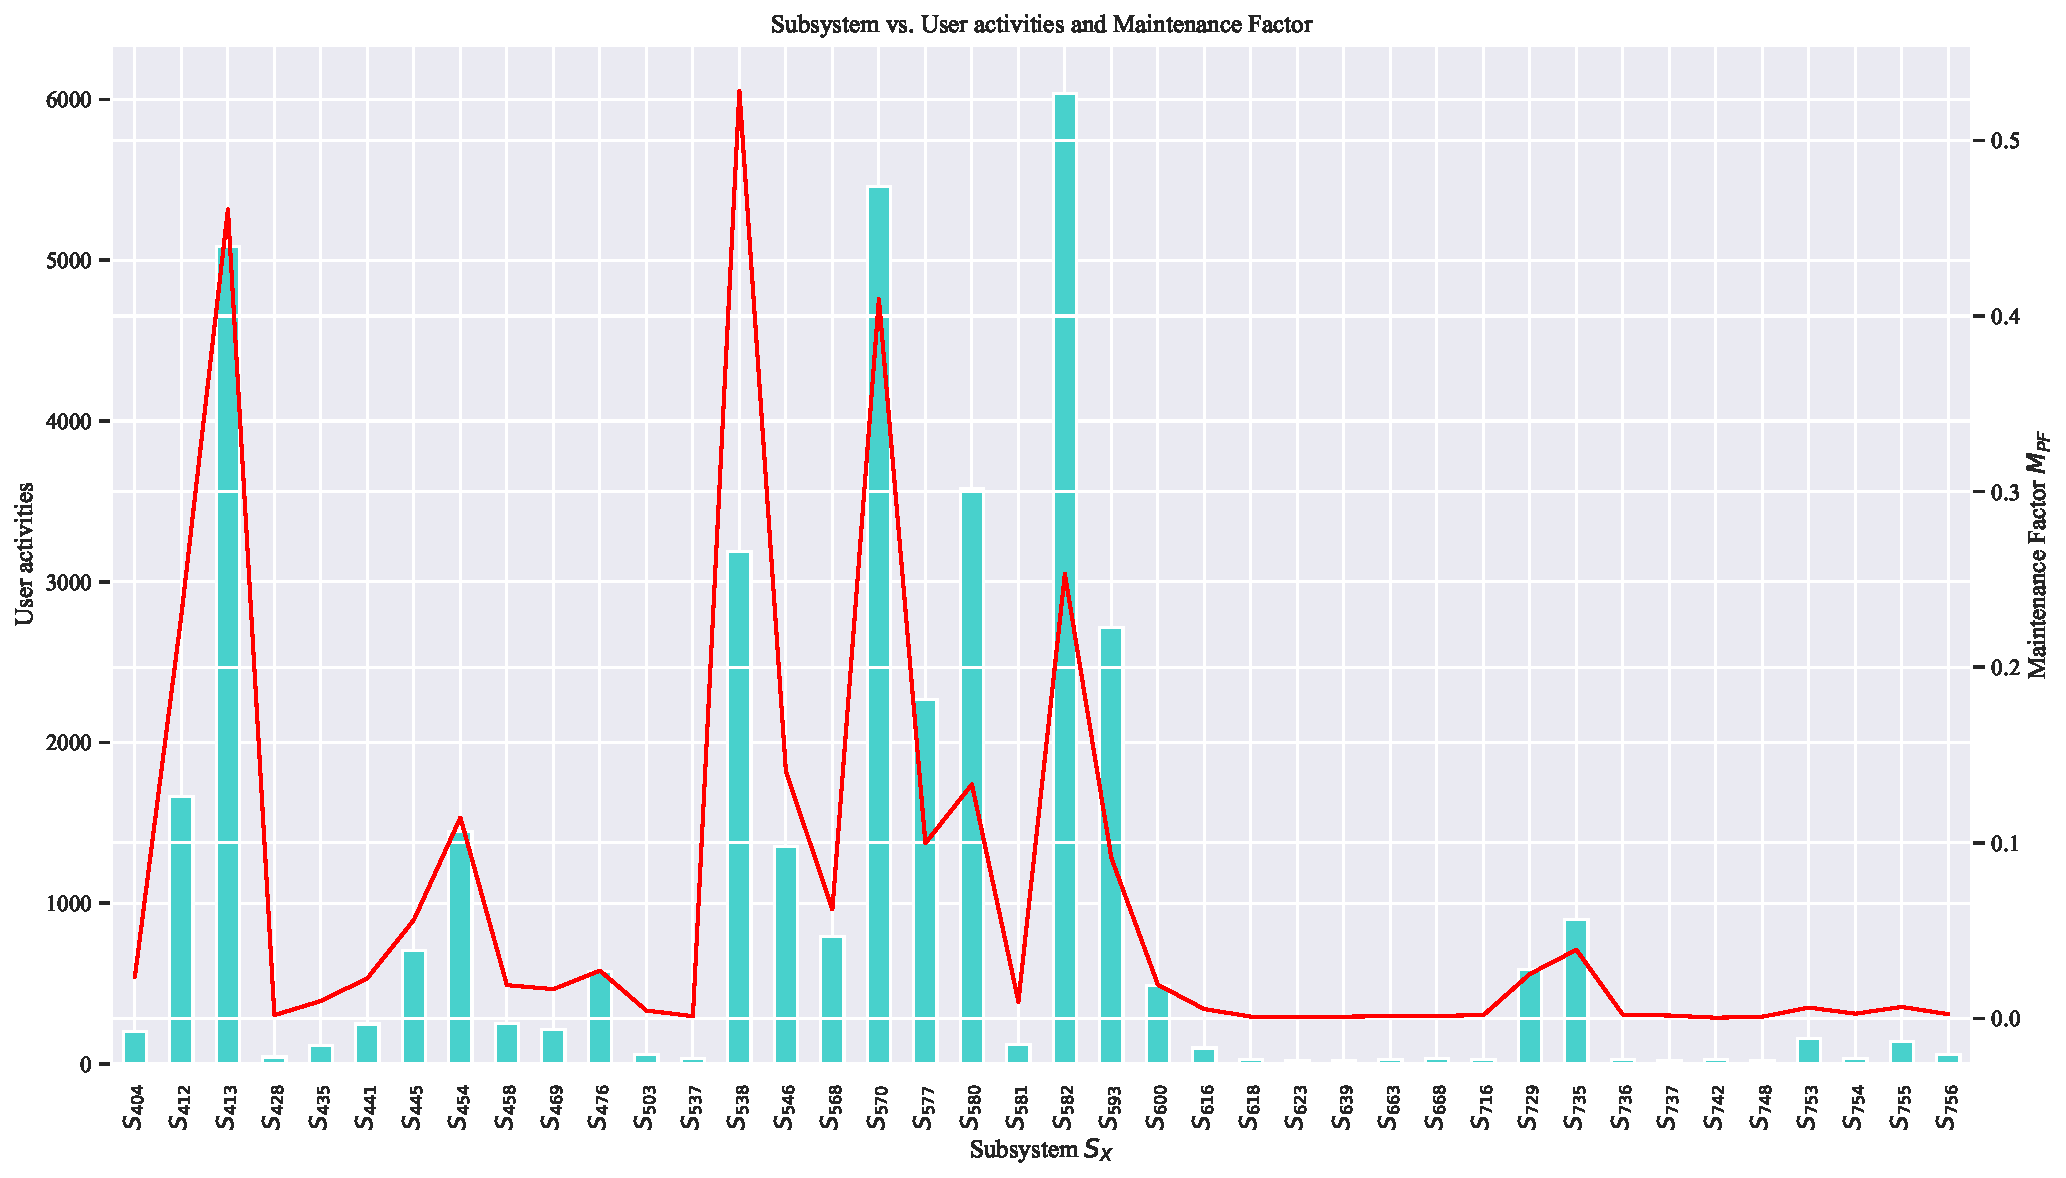
\includegraphics[width=0.95\linewidth]{img/ch3/analysis/case_A_subsystems_1.pdf}
		\caption[Case study 1 subsystem activities part 1]
		{\textit{Case study 1 subsystem activities part 1}}\label{fig:ch3_saS1S246}
	\end{figure} 
\end{landscape}

\subsubsection{System B results}

\clearpage

\subsection{Critical analysis results}

\section{Conclusion}